\documentclass[letterpaper]{article}
\usepackage{natbib}
\usepackage[utf8]{inputenc}
\usepackage{graphicx}
\usepackage{color}
\usepackage{multirow}
\usepackage{amsmath}
\usepackage{array}
\usepackage{subcaption}
\usepackage{mathpazo}
\usepackage[a4paper]{geometry}

\title{Learning Dynamics: Assignment 2}
\author{\Large Hakim Boulahya \\
hboulahy@ulb.ac.be\\
\\
Université Libre de Bruxelles
}

\begin{document}
\maketitle
\tableofcontents
\newpage
\section{Part I}

% Coop level for 50
\begin{figure}
    \begin{subfigure}{.5\textwidth}
        \centering
        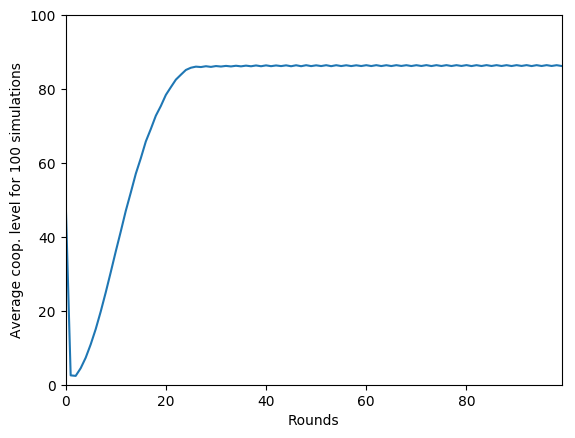
\includegraphics[width=1\linewidth]{images/assign2/50-part1}
        \caption{Moore neighborhood}
        \label{fig:50moorepart1}
    \end{subfigure}
    \begin{subfigure}{.5\textwidth}
        \centering
        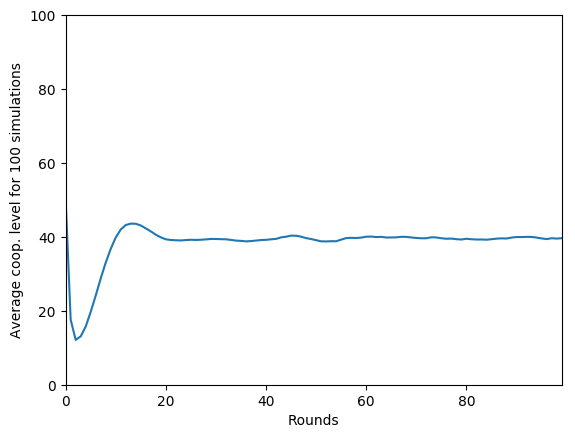
\includegraphics[width=1\linewidth]{images/assign2/50_vonneumann-part1}
        \caption{Von Neumann neigborhood}
        \label{fig:50vonpart1}
    \end{subfigure}
    \caption{Cooperation level using unconditional imitation and
    weak prisoner's dilemma on a 50x50 lattice}
    \label{fig:50part1}
\end{figure}

% Visualization for 50

\begin{figure}
    \begin{subfigure}{.3\textwidth}
      \centering
      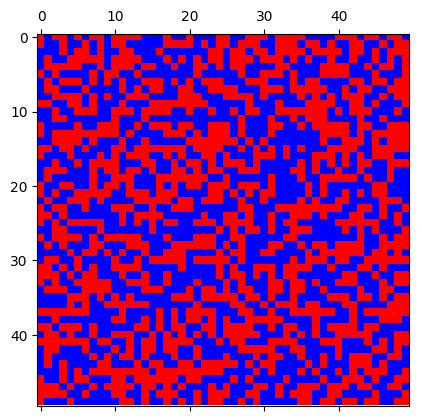
\includegraphics[width=1\linewidth]{images/assign2/visu_50-part1/t0}
      \caption{$t_0$}
      \label{fig:t0_50part1}
    \end{subfigure}
    \begin{subfigure}{.3\textwidth}
      \centering
      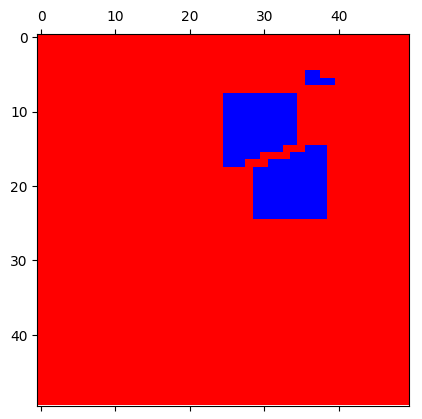
\includegraphics[width=1\linewidth]{images/assign2/visu_50-part1/t5}
      \caption{$t_5$}
      \label{fig:t5_50part1}
    \end{subfigure}
    \begin{subfigure}{.3\textwidth}
      \centering
      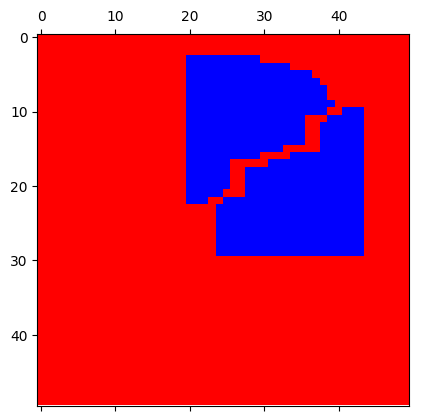
\includegraphics[width=1\linewidth]{images/assign2/visu_50-part1/t10}
      \caption{$t_{10}$}
      \label{fig:t10_50part1}
    \end{subfigure}
    \begin{subfigure}{.3\textwidth}
      \centering
      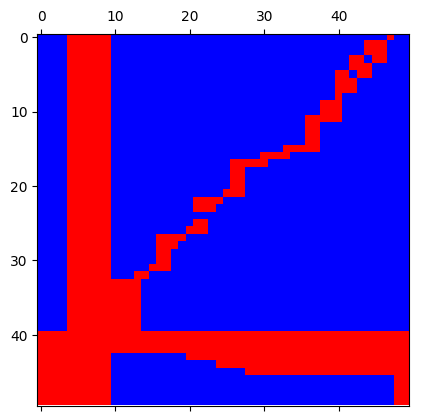
\includegraphics[width=1\linewidth]{images/assign2/visu_50-part1/t20}
      \caption{$t_{20}$}
      \label{fig:t20_50part1}
    \end{subfigure}
    \begin{subfigure}{.3\textwidth}
      \centering
      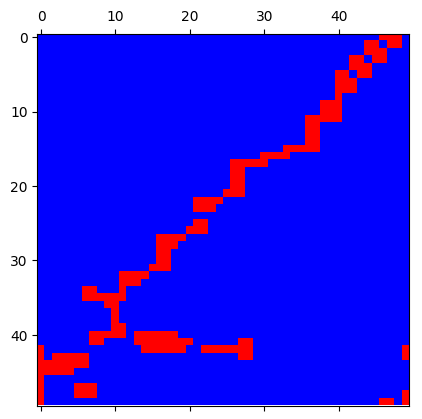
\includegraphics[width=1\linewidth]{images/assign2/visu_50-part1/t50}
      \caption{$t_{50}$}
      \label{fig:t50_50part1}
    \end{subfigure}
    \caption{Visualization of a the lattice with unconditional imitation,
    Moore neighborhood and weak prisoner's, dilemma}
    \label{fig:visu50part1}
\end{figure}

% Coop level for all others
\begin{figure}
    \begin{subfigure}{.5\textwidth}
        \centering
        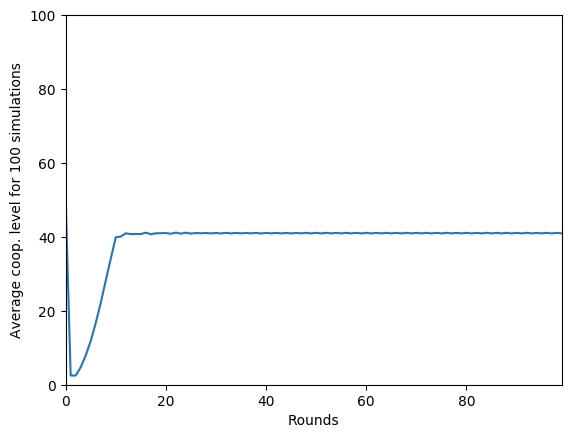
\includegraphics[width=1\linewidth]{images/assign2/20-part1}
        \caption{20x20}
        \label{fig:20moorepart1}
    \end{subfigure}
    \begin{subfigure}{.5\textwidth}
        \centering
        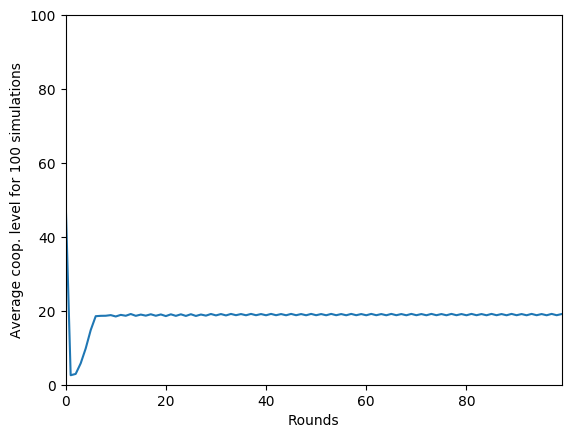
\includegraphics[width=1\linewidth]{images/assign2/12-part1}
        \caption{12x12}
        \label{fig:12moorepart1}
    \end{subfigure}
    \begin{subfigure}{.5\textwidth}
        \centering
        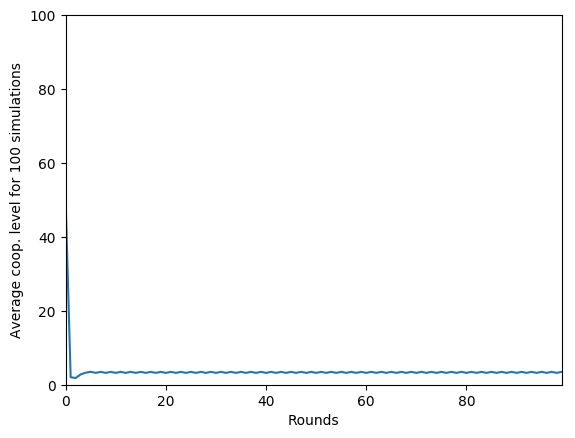
\includegraphics[width=1\linewidth]{images/assign2/8-part1}
        \caption{8x8}
        \label{fig:8moorepart1}
    \end{subfigure}
    \begin{subfigure}{.5\textwidth}
        \centering
        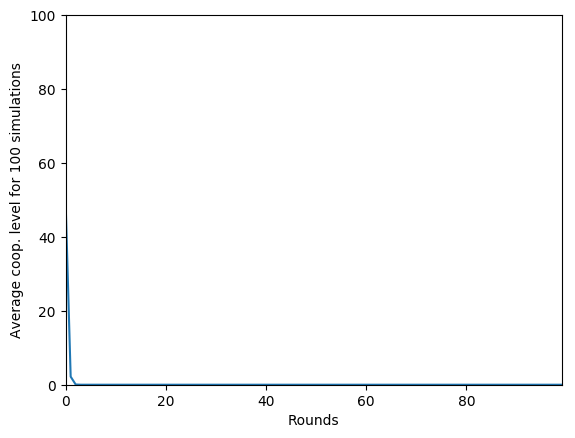
\includegraphics[width=1\linewidth]{images/assign2/4-part1}
        \caption{4x4}
        \label{fig:4moorepart1}
    \end{subfigure}
    \caption{Cooperation level using unconditional imitation, Moore neighborhood
    and weak prisoner's dilemma}
    \label{fig:otherpart1}
\end{figure}

\section{Part II}

% Coop level for 50
\begin{figure}
    \begin{subfigure}{.5\textwidth}
        \centering
        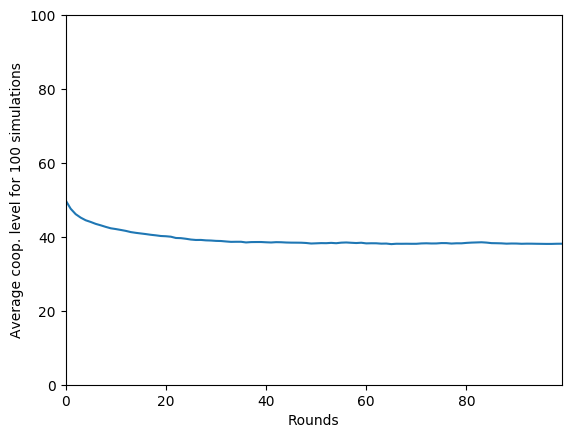
\includegraphics[width=1\linewidth]{images/assign2/50-part2}
        \caption{Moore neighborhood}
        \label{fig:50moorepart2}
    \end{subfigure}
    \begin{subfigure}{.5\textwidth}
        \centering
        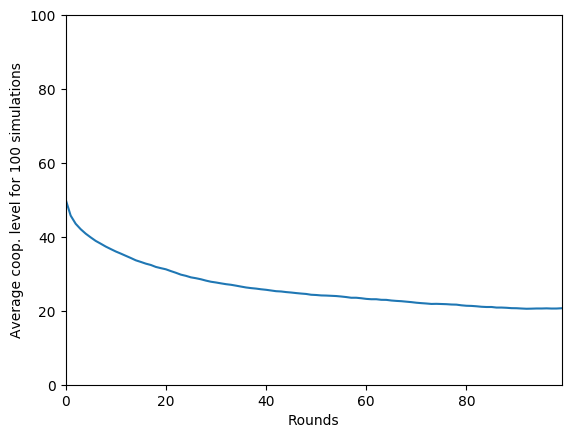
\includegraphics[width=1\linewidth]{images/assign2/50_vonneumann-part2}
        \caption{Von Neumann neigborhood}
        \label{fig:50vonpart2}
    \end{subfigure}
    \caption{Cooperation level using replicator rule and
    snowdrift game on a 50x50 lattice}
    \label{fig:50part2}
\end{figure}

% Visualization for 50
\begin{figure}
    \begin{subfigure}{.3\textwidth}
      \centering
      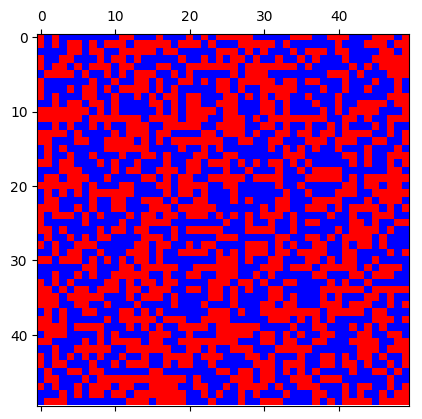
\includegraphics[width=1\linewidth]{images/assign2/visu_50-part2/t0}
      \caption{$t_0$}
      \label{fig:t0_50part2}
    \end{subfigure}
    \begin{subfigure}{.3\textwidth}
      \centering
      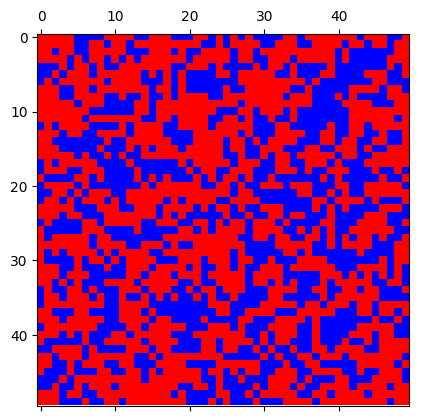
\includegraphics[width=1\linewidth]{images/assign2/visu_50-part2/t5}
      \caption{$t_5$}
      \label{fig:t5_50part2}
    \end{subfigure}
    \begin{subfigure}{.3\textwidth}
      \centering
      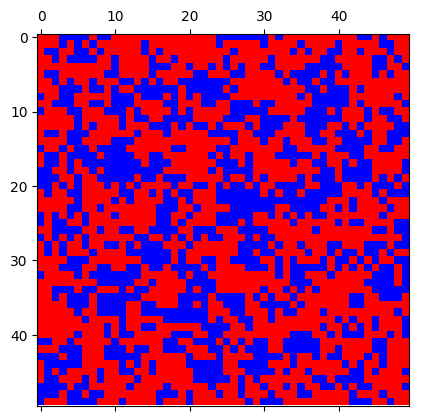
\includegraphics[width=1\linewidth]{images/assign2/visu_50-part2/t10}
      \caption{$t_{10}$}
      \label{fig:t10_50part2}
    \end{subfigure}
    \begin{subfigure}{.3\textwidth}
      \centering
      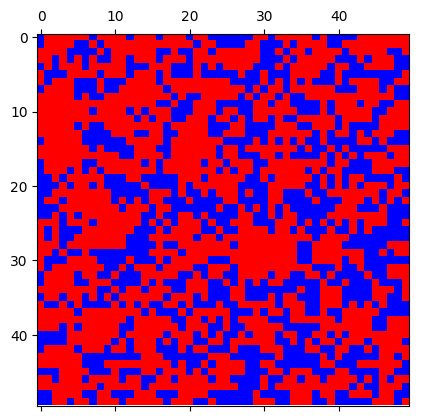
\includegraphics[width=1\linewidth]{images/assign2/visu_50-part2/t20}
      \caption{$t_{20}$}
      \label{fig:t20_50part2}
    \end{subfigure}
    \begin{subfigure}{.3\textwidth}
      \centering
      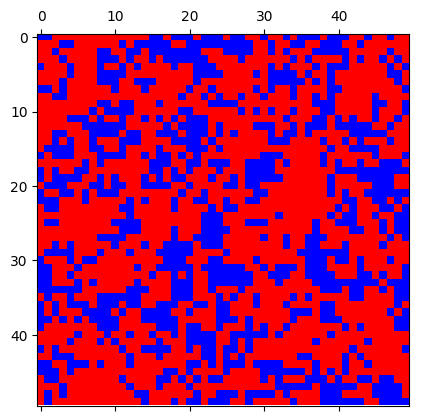
\includegraphics[width=1\linewidth]{images/assign2/visu_50-part2/t50}
      \caption{$t_{50}$}
      \label{fig:t50_50part2}
    \end{subfigure}
    \caption{Visualization of a the lattice with replicator rule,
    Moore neighborhood and snowdrift game}
    \label{fig:visu50part2}
\end{figure}

% Coop level for all others
\begin{figure}
    \begin{subfigure}{.5\textwidth}
        \centering
        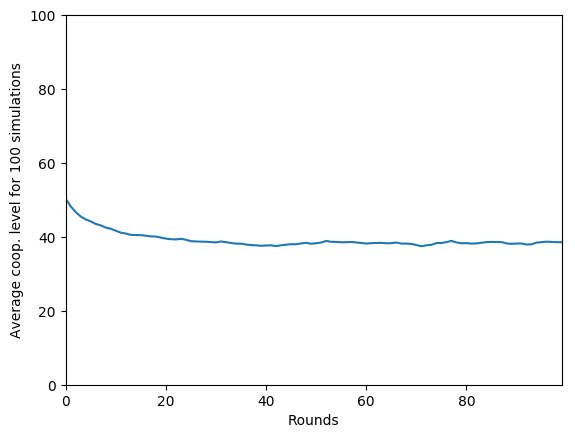
\includegraphics[width=1\linewidth]{images/assign2/20-part2}
        \caption{20x20}
        \label{fig:20moorepart2}
    \end{subfigure}
    \begin{subfigure}{.5\textwidth}
        \centering
        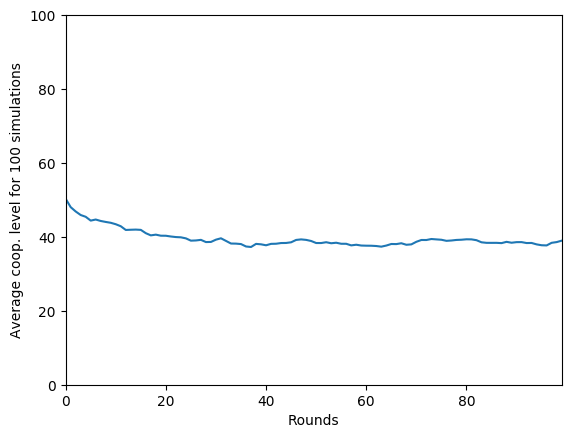
\includegraphics[width=1\linewidth]{images/assign2/12-part2}
        \caption{12x12}
        \label{fig:12moorepart2}
    \end{subfigure}
    \begin{subfigure}{.5\textwidth}
        \centering
        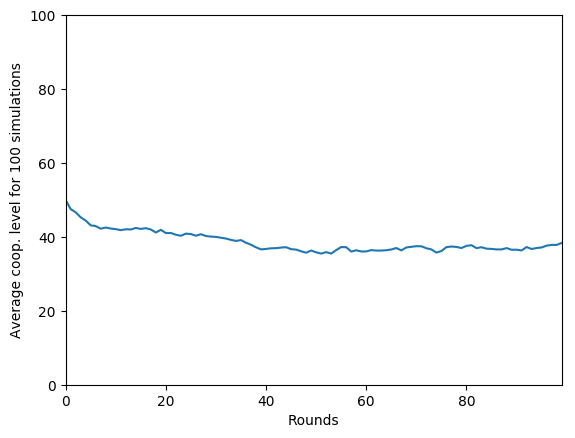
\includegraphics[width=1\linewidth]{images/assign2/8-part2}
        \caption{8x8}
        \label{fig:8moorepart2}
    \end{subfigure}
    \begin{subfigure}{.5\textwidth}
        \centering
        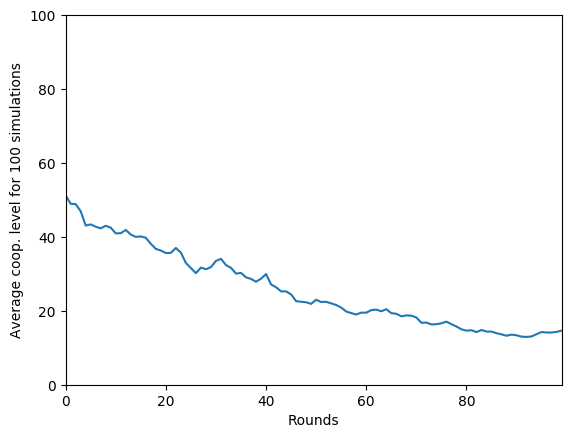
\includegraphics[width=1\linewidth]{images/assign2/4-part2}
        \caption{4x4}
        \label{fig:4moorepart2}
    \end{subfigure}
    \caption{Cooperation level using replicator rule, Moore neighborhood
    and snowdrift game}
    \label{fig:otherpart2}
\end{figure}


\end{document}
